\documentclass[handout]{beamer}
\usepackage{tikz}
\usepackage[utf8]{inputenc}
\usepackage{subcaption}
\usepackage{colortbl}
\graphicspath{{./}{images/}}
\usetheme{default}
\title{Programmation CUDA}
\author{S. Puechmorel}
\date{2023}

\pgfdeclareimage[interpolate=true, height=0.155\paperwidth,width=\paperwidth]{bloc_enac}{images/Bloc_marque_RF_ENAC_V2.png}
\pgfdeclareimage[interpolate=true, height=40pt]{bloc2_enac}{images/Bloc_marque_RF_ENAC_V1.png}
\setbeamertemplate{background}{
  \begin{tikzpicture}
    \ifnum\thepage=1%
  \useasboundingbox (0,0) rectangle (\the\paperwidth,\the\paperheight); 
    \pgftext[at=\pgfpoint{0}{\paperheight-0.155\paperwidth},left,base]{\pgfuseimage{bloc_enac}};
    \else
\useasboundingbox (0,0) rectangle (\the\paperwidth,\the\paperheight); 
    \pgftext[at=\pgfpoint{0}{\paperheight-40pt},left,base]{\pgfuseimage{bloc2_enac}};
    \fi

  \end{tikzpicture}
}

\setbeamertemplate{frametitle}{
 \ifnum\thepage>1%
  \rightline{\insertframetitle}
 \fi   
}

\begin{document}
%1
\begin{frame}
    \titlepage

\end{frame}
%2
\begin{frame}
  \frametitle{Plan}
\tableofcontents
\end{frame}
\section{Historique}
%3
\begin{frame}
    \frametitle{L'évolution des cartes graphiques.}
\begin{block}{Années 1980 : contrôleurs video.}
  Ces circuits permettaient d'afficher sur un tube cathodique 
  des informations stockées en mémoire. Ils fournissaient des fonctionnalités de base, essentiellement orientées
  autour de la gestion de la mémoire vidéo et de la génération des signaux de synchronisation. 
  \begin{figure}[ht]
    \centering
    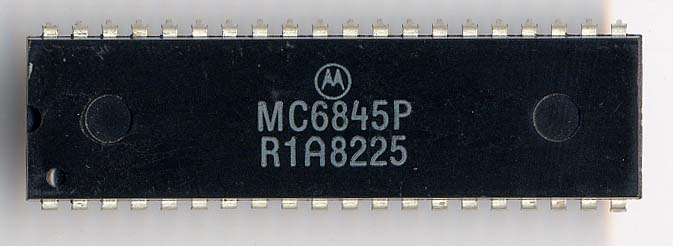
\includegraphics[scale=0.5]{Motorola_MC6845.jpg}
    \caption{Le contrôleur vidéo MC6845. \footnote{\tiny \url{https://commons.wikimedia.org/w/index.php?curid=976920}}}
    \label{fig:MC6845}
  \end{figure}
\end{block}
\end{frame}
%4
\begin{frame}
  \frametitle{L'évolution des cartes graphiques.}
\begin{block}{Contrôleurs graphiques}
  Apparus vers la fin des années 1980, ils apportent des fonctionnalités graphiques, telles le tracé de segment, 
  et gèrent une mémoire distincte de celle de l'unité centrale.
   \begin{figure}[htbp]
    \centering
    \hfill
   \begin{subfigure}{0.4\textwidth}
    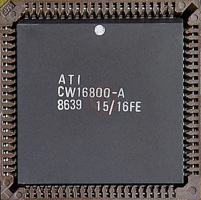
\includegraphics[scale=0.45]{ATI16800.jpg}
   \end{subfigure} 
   \hfill
   \begin{subfigure}{0.4\textwidth}
    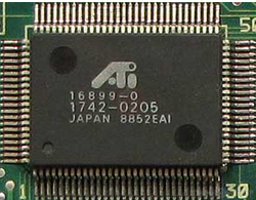
\includegraphics[scale=0.45]{ATI16899.jpg}
   \end{subfigure} 
   \hfill
    \caption{Contrôleurs graphiques.}
    \label{fig:graphic_controllers}
   \end{figure}
\end{block}
\end{frame}
%5
\begin{frame}
  \frametitle{L'évolution des cartes graphiques.}
\begin{block}{Les processeurs graphiques 3D.}
    Disponibles pour le grand public depuis le milieu des années 1990, ils incluent des fonctionalités
    d'affichage en trois dimensions. Parallèlement, des bibliothèques logicielles font leur apparition
    (OpenGL, Direct3D). L'affichage d'une scène est réalisé à travers un pipeline graphique: 
    transformation de sommets, projection, traçage.
    \begin{figure}[htbp]
        \centering
       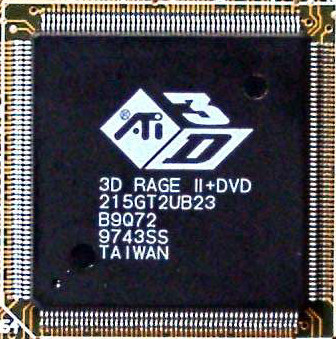
\includegraphics[scale=0.2]{3drage.jpg} 
        \caption{Contrôleur 3D ATI Rage.}
        \label{fig:ati_rage}
    \end{figure}
\end{block}
\end{frame}
%6
\begin{frame}
  \frametitle{L'évolution des cartes graphiques.}
\begin{block}{Les processeurs progammables.}
    En 2001, la société NVIDIA introduit sur le marché la gamme de processeurs graphiques
    GeForce 3 qui permettent de programmer les étapes du pipeline graphique. 
    \begin{figure}[htbp]
        \centering
       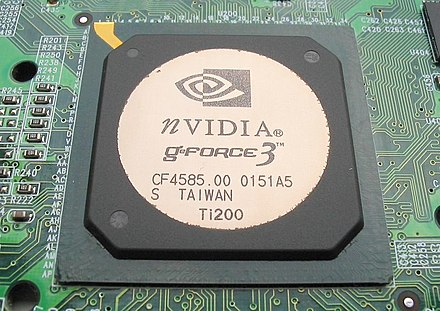
\includegraphics[scale=0.3]{Geforce3gpu.jpg} 
        \caption{Contrôleur 3D programmable.}
        \label{fig:geforce3}
    \end{figure}
\end{block}
%7
\end{frame}

\begin{frame}
  \frametitle{L'évolution des cartes graphiques.}
\begin{block}{Le calcul.}
    Fin 2006, NVIDIA lance la gamme GeForce 8 et l'environnement de développement CUDA qui
    permet d'exploiter la puissance de calcul des cartes graphiques pour des applications générales.
    Les performances théoriques sont impressionnantes, de l'ordre de celles obtenues avec un 
    superordinateur pour uen enveloppe énergétique comparable.

    \begin{figure}[htbp]
        \centering
       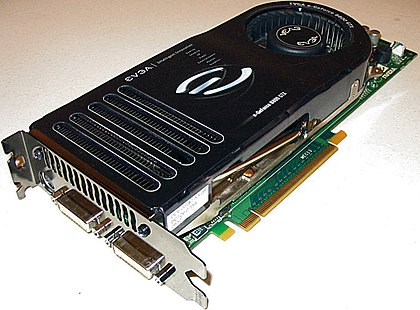
\includegraphics[scale=0.3]{geforce8800.jpg} 
        \caption{Carte graphique CUDA.}
        \label{fig:gforce8}
    \end{figure}
\end{block}
\end{frame}

\begin{frame}
  \frametitle{Synthèse de l'évolution des cartes NVIDIA}
{\footnotesize  
\hspace{-1cm}
            \begin{tabular}{p{3cm}p{1.5cm}p{3.5cm}p{1cm}p{1cm}p{1cm}}
            \rowcolor{lightgray}\textbf{Année} & \textbf{Carte} & \textbf{Architecture} & \textbf{Cœurs NVIDIA CUDA} & \textbf{RAM} & \textbf{Puissance} \\\hline
            1995 & NV1 & dizaines de micromètres (µm) & ?  & 2-4 Mo & 2 Watts \\
            ... & ... & ...  & ... & ... & ...\\
    
            2017 & GTX 1080 Ti & Volta 16 nm & 1920 & 11 Go & 257 watts \\
            2019 & GTX 2080 Ti & Turing 12 nm & 1920 & 11 Go & 290 Watts \\
            2020 & RTX 3090 & Ampere 8 nm & 10 496 & 24 Go & 350 Watts \\
            2022 & RTX 4090 & Ada Lovelace 4 nm & 18 000  & 24 Go & 450-600 Watts \\            
        \end{tabular}
\end{block}
\end{frame}

\section{Architecture des GPUs}
%1
\begin{frame}
    \frametitle{Architecture matérielle}
\begin{block}{Les multiprocesseurs de flux (SM)}
   \begin{itemize}
    \item<+-> Héritier du pipeline graphique, le multiprocesseur de flux ("Streaming multiprocessor", SM) 
    est une entité de traitement comportant des séquenceurs, plusieurs unités de traitement numérique et une mémoire locale.
    \item<+-> Un processeur graphique (GPU) regroupe plusieurs multiprocesseurs. 
    \item<+-> Les multiprocesseurs exécutent des blocs de processus de façon \textbf{indépendante} et peuvent accéder à
    une mémoire partagée.
    \item<+-> Pour un développeur sur une architecture conventionnelle, un multiprocesseur s'apparente à un c{\oe}ur de calcul
    vectoriel.
   \end{itemize} 
\end{block}
    

\end{frame}
%2
\begin{frame}
    \frametitle{Architecture matérielle}
\begin{block}{Les multiprocesseurs de flux (SM)}
   \begin{itemize}
    \item<+->À l'intérieur d'un multiprocesseur, les processus s'exécutent de façon concurrente, mais peuvent communiquer
    via la mémoire locale ou être synchronisés.
    \item<+->Les processus sont regroupés par blocs, appelés "warps" (chaînes), qui se voient affecter le même séquenceur 
    d'instructions.
    \item<+->Le modèle associé est dit "SIMT" pour "Single Instruction Multiple Thread".
   \end{itemize} 
\end{block}
\end{frame}
x
%3
\begin{frame}
    \frametitle{Architecture matérielle}
\begin{block}{Les unités de calcul}
   \begin{itemize}
    \item<+-> Le nombre d'unités de calcul par multiprocesseur dépend des générations de cartes. Pour l'architecture 
    Ampère, on trouve 64 ou 128 unités flottantes 32bits, 32 ou 2 unités flottantes 64bits, 64 unités de calcul entier
    sur 32 bits, 16 unités spéciales (fonctions transcendantes), 4 cœurs de calcul tensoriel et 4 ordonnanceurs.
    \item<+-> Un ordonnanceur est affecté à une chaîne. Tous les processus de la chaîne exécutent la même Instruction
    au même moment.
    \item<+-> En cas d'instruction conditionnelle, il peut y avoir divergence de code à l'intérieur d'une chaîne, ce qui se traduit par la 
    mise en attente d'un ou plusieurs processus dont l'exécution se poursuivra après celle de la branche principale. 
   \end{itemize} 
\end{block}
\end{frame}
\begin{frame}
    \frametitle{Architecture matérielle}
\begin{block}{L'ordonnancement des processus}
   \begin{itemize}
    \item<+-> Le code à exécuter sur le GPU est appelé noyau ("kernel".)
    \item<+-> Le programmeur décide du nombre de processus affectés à un même noyau et les répartit en blocs.
    \item<+-> Un bloc sera pris en charge par un multiprocesseur libre.
    \item<+-> Dans un bloc, des chaînes de 32 processus identifiés par des entiers consécutifs sont constituées. 
    \item<+-> Depuis l'architecture Volta, chaque processus possède ses propres compteur de programme et pile d'appel,
    ce qui permet un contrôle plus fin, en particulier en cas de divergence.
   \end{itemize} 
\end{block}
\end{frame}
%4
\begin{frame}
    \frametitle{Architecture matérielle}
\begin{block}{La mémoire}
   \begin{itemize}
    \item<+-> Chaque multiprocesseur possède une mémoire locale très rapide, pouvant être partagée entre les processus
    d'un même bloc. Elle est organisée en 32 banques pouvant être utilisées simultanément. Idéalement, 
    chaque processus d'une chaîne accède à sa propre banque. La capacité de cette mémoire varie entre 64kB et 228kB 
    selon les générations.
    \item<+-> Les multiprocesseurs partagent une mémoire globale, plus lente, mais en mesure de stocker beaucoup plus 
    de données. Les cartes de dernière génération, comme la RX4090, embarquent 24Gb de RAM.
    \item<+-> L'architecture 9.0 introduit la notion de cluster de blocs et de mémoire partagée distribuée.
   \end{itemize} 
\end{block}
\end{frame}
\begin{frame}{Les mémoires spécialisées}
\begin{block}{La mémoire de textures}
   \begin{itemize}
    \item<+-> Les GPUs étant initialement conçus pour des applications de rendu graphique 3D, certaines mémoires
    dédiées sont présentes. 
    \item<+-> La mémoire de textures est particulièrement intéressante lorsque l'on cherche à stocker des données
    bidimensionnelles que l'on souhaite ensuite interpoler.
    \item<+-> Cette mémoire, chargée par le CPU, ne peut être modifiée par un programme CUDA.
   \end{itemize} 
\end{block}
\end{frame}
\begin{frame}{\`A retenir}
\begin{block}{Le GPU}
   \begin{itemize}
    \item<+-> Un bloc est affecté à un multiprocesseur, les processus d'une même chaîne exécutent la même Instruction
    en parallèle.
    \item<+-> Il faut donc penser avant tout en termes de chaînes (32 processus).
    \item<+-> Un branchement dans un même chaîne entraîne l'inactivation temporaire de processus.
   \end{itemize} 
\end{block}
\begin{block}{La mémoire}
  \begin{itemize}
   \item<+-> Privilégier l'utilisation de la mémoire partagée, bien plus rapide que la mémoire globale.
   \item<+-> S'efforcer d'avoir des accès contigus pour les processus d'une même chaîne.
   \item<+-> Penser à utiliser la mémoire des textures si nécessaire.
  \end{itemize} 
\end{block}
\end{frame}

\end{document}
